\subsection{Reports generated in the software}
Following are the reports generated in TCC Automation software :
\begin{itemize}
\item {\bf{ Suspence Report:}} This report keep record of all the suspence jobs that has been registered.
\item {\bf{Suspence-Clearance Report:}} This report is used to get all te suspence registered jobs whose dues have been cleared out.
\item {\bf {T.A./D.A. Bill:}} This is report for Transport Allowance and Daily Allowance bill.
\item {\bf {Performa Bill:}} It give the 
\item {\bf {Job Register:}} It keep record of all the jobs registered.
\item {\bf {Yearly/Monthly Income Report:}} It gives the yearly and monthly record of income to the institute.
\item {\bf {Transport Bill:}} It gives all the information related to transportation.
\item {\bf {Other charge Bill:}} It gives the report of all the other charges like service tax, education tax, etc.
\item {\bf {Daily report:}} It gives the information of job registered in  the number of days selected. It also makes the differance between the types of payments made like cheque, cash.
\item {\bf {Faculty Income distribution:}} It keeps the record of the income distribution to the faculty members.
\item {\bf {Main Register:}} It is the main register keeping the record of all the report types.
\item {\bf {Receipt:}} It keeps te record of all the recieps. One only need to know the job no. and then can easily get the receipt.
\item {\bf {Department/lab Report:}} It carries all the information of various labs and thus gives the record for the lab selected.
\item {\bf {Govt./Semi-Govt./Private Report:}} It keeps the record for the type of work selected i.e Govt./Semi-Govt./Private Report.
\item {\bf {Clearance Report:}} It gives the clearance report.
\item {\bf {General Bill:}} It keeps record of all the general reports.
\end{itemize}
\newpage
\begin{figure}[h]
\centering \includegraphics[scale=0.7]{a1.png}
\caption{Bill Report}
\end{figure}
\newpage
\begin{figure}[h]
\centering \includegraphics[scale=0.7]{a2.png}
\caption{General Clearance Report}
\end{figure}
\newpage
\begin{figure}[h]
\centering \includegraphics[scale=0.7]{a3.png}
\caption{Suspense Clearance Report}
\end{figure}
\newpage


\subsection{Distribution of money}
\begin{itemize}
\item College Income
\item Administrative
\item Development Funds
\item Consultatancy Asst.
\item Service Tax
\item Education Tax
\item Higher-Education Tax
\end{itemize}
\newpage
\subsection{My Contribution to the project}
\begin{itemize}
\item Made Login and registration application
\item Added a report named `Daily Report'
\item Added a module named `Labs'
\item Introduced new tables in admin section
\item Gave different database permissions to different staff members\\
\end{itemize}

\newpage
\begin{description}
\item[Login Application] : This application allows one register oneself in the software and use it by logging in. This increased the security of the project as now only the authorised users can have access to the software and thus use it. Any unauthorised user now cannot misuse it.
\end{description}
\begin{figure}[h]
\centering 
\includegraphics[scale=0.3]{Screenshot.png}
\caption{Login application introduced in software}
\end{figure}
\newpage
\begin{description}
\item[Daily Report module] : It was not possible earlier to have a record amount of a day in TCC or number of number of days selected but after introduction of this module in the software one can do so. This has moreover increased the level of automation.
Also it can make the differanc between the type of payment made. That means now on can have record of cash and cheques payments making the users easy to handle the work.
\end{description}


\begin{figure}[h]
\centering \includegraphics[scale=0.4]{s1.png}
\caption{Daily Report module added}
\end{figure}
\begin{figure}[h]
\newpage
\centering 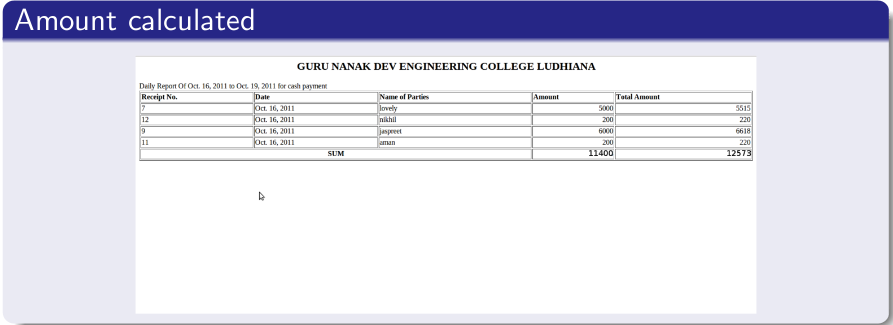
\includegraphics[scale=0.4]{dp3.png}
\caption{Cash type selected to make selection for report}
\end{figure} 
\begin{figure}[h]
\centering 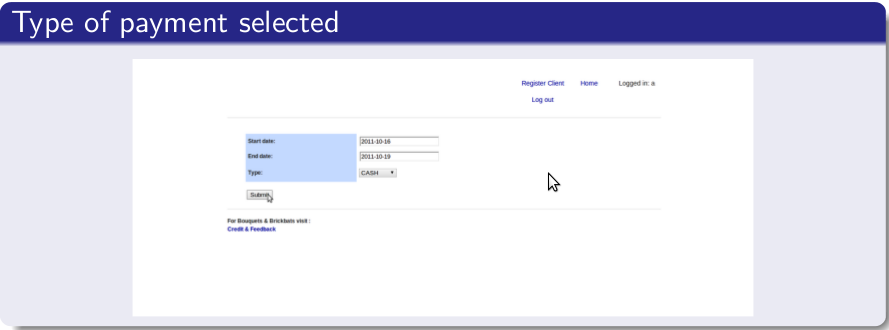
\includegraphics[scale=0.4]{dp4.png}
\caption{Report for cash payment for number of days selected}
\end{figure} 
\begin{description}
\newpage
\item[Labs module] : This module is used to find the amount recieved for a particular lab for the number of days selected. It gives the record for the labs in TCC for number of days selected. It has also automated the work.
\end{description}
\begin{figure}[h]
\centering \includegraphics[scale=0.4]{s4.png}
\caption{labs module added}
\end{figure}
\newpage
\vspace{5cm}
\begin{figure}[h]
\centering 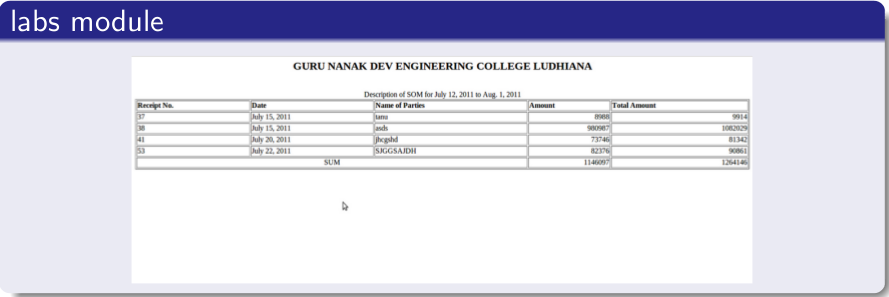
\includegraphics[scale=0.4]{lb1.png}
\caption{Amount recieved for the lab in number of days selected}
\end{figure}
\newpage
\begin{description}
\item[Introduction of new tables in admin] : Introduction of new tables in admin has made the admin of software more powerful as now in order to change the database entries he can directly make changes by going to these tables. This made the interface of user with the software easier, without getting tracked in the datbase tables and codings.
\end{description}
\begin{figure}[h]
\centering 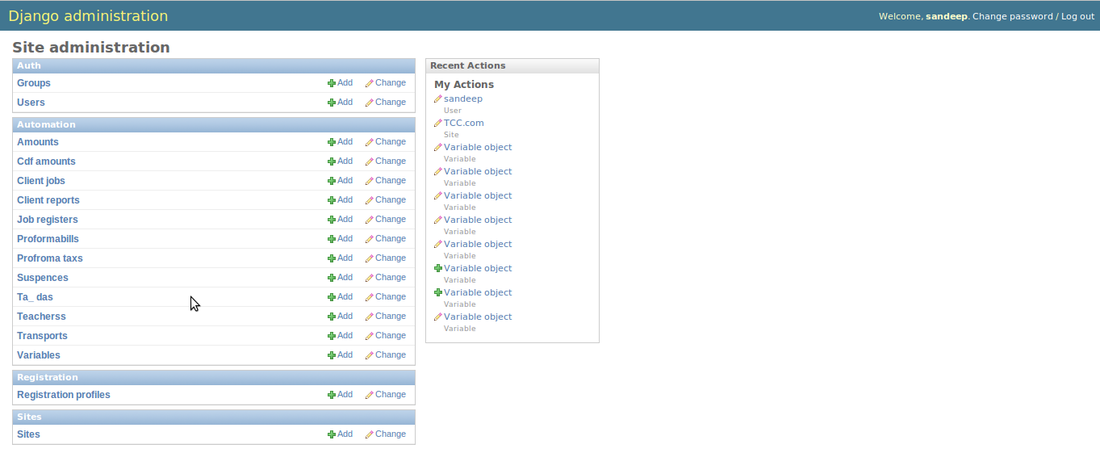
\includegraphics[scale=0.4]{s5.png}
\caption{Automation tables added in admin}
\end{figure}
\newpage
\subsection{Advantages of Automation}
\begin{itemize}
\item Great way to save money.
\item Reduce paper work.
\item Automatic calculations.
\item Less man power.
\item Increased efficiency.
\item Increased Accuracy.
\item Less time for protecting information.
\item Handle a work more faster.
\item Backup record.
\item Easy transformation.
\item Easy management.
\item Less storage space is required.
\item Overall development of system.
\item Minimize error and processing.
\end{itemize}
